%%%%%%%%%%%%%%%%%%%%%%%%%%%%%%%%%%%%%%%%%%%%%%%%%%%%%%%%%%%%%%%%%%%%%%%%%
%%%  ISWC 2017 - CityMUS: Music Recommendation When Exploring a City  %%%
%%%%%%%%%%%%%%%%%%%%%%%%%%%%%%%%%%%%%%%%%%%%%%%%%%%%%%%%%%%%%%%%%%%%%%%%%

\documentclass{llncs}

\usepackage{url}
\usepackage{graphicx}
\usepackage{xtab}
\usepackage{xfrac}
\usepackage[inline]{enumitem}
\DeclareGraphicsExtensions{.png}

\newcommand\figref{Figure~\ref}
\newcommand\tabref{Table~\ref}

%% Save the class definition of \subparagraph
\let\llncssubparagraph\subparagraph
%% Provide a definition to \subparagraph to keep titlesec happy
\let\subparagraph\paragraph
\usepackage{titlesec}
%% Revert \subparagraph to the llncs definition
\let\subparagraph\llncssubparagraph

\titleformat{\subsection}[runin]{\bfseries}{}{}{}[]

%%%%%%%%%%%%%%%%%%%%%%%%%%%%%%%
%%%  Beginning of document  %%%
%%%%%%%%%%%%%%%%%%%%%%%%%%%%%%%

\begin{document}

\title{CityMUS: Music Recommendation\\When Exploring a City}

\author{Pasquale Lisena\inst{1} \and
Lorenzo Canale\inst{1} \and Fabio Ellena\inst{1}
\and Rapha\"el Troncy\inst{1}}
\authorrunning{Lisena and al.}
\institute{EURECOM, Sophia Antipolis, France \\
\email{\{lisena|canale|ellena|troncy\}@eurecom.fr}}

\maketitle

%%%%%%%%%%%%%%%%%%
%%%  Abstract  %%%
%%%%%%%%%%%%%%%%%%

\begin{abstract}
Linked Data makes possible the discovery of interesting connections between semantic entities that belong to different domains. This paper presents CityMUS, a web application that gives to the user the experience of a walk in the city with the most suitable soundtrack, on the base of the urban context. The application relies on a recommender system that searches for paths in a knowledge graph between nearby places and music composers, making use of a combination of DBpedia and domain-specific datasets.
\end{abstract}

%%%%%%%%%%%%%%%%%%%%%%%%%%%%%%%%%%%%%%%%%%%%%%%%%%%%%
%%%  1. Recommending Music in Urban Environments  %%%
%%%%%%%%%%%%%%%%%%%%%%%%%%%%%%%%%%%%%%%%%%%%%%%%%%%%%

\section{Recommending Music in Urban Environments}
\label{sec:introduction}
The consumption of music content on the move is one of the hottest trends. Some projects have sought to combine the experience of exploring a city with the one of media consumption~\cite{braunhofer2013location,perez2015geolocation}.  Context-based recommendation of music can be obtained using Linked Data. A strategy consists in exploiting arbitrary semantic connection between \textit{Points of Interest (PoIs)} and musicians using knowledge graphs such as DBpedia, defining in this way a similarity measure between these two different domains~\cite{kaminskas2012knowledge}. So far, the implementation of this strategy relies on domain experts' who select a subset of classes used in the graph and manually define the interesting connection (i.e. path of properties), giving them a weight that can be used in a recommendation algorithm.

In this paper, we propose a completely unsupervised approach for developing a music recommendation system based on nearby PoIs. This strategy relies on the combination of general and encyclopedic datasets (i.e. DBpedia) and specialised datasets. We chose the city of Nice as an example for performing our experiment\footnote{The demo is publicly available at \url{https://citymus.doremus.org/} while the source code is at \url{https://github.com/MultimediaSemantics/CityMUS}}.

%%%%%%%%%%%%%%%%%%%%%%%%%%%%%%%%%%%%%%%%%%%%%
%%%  2. Data Preparation and Path Finder  %%%
%%%%%%%%%%%%%%%%%%%%%%%%%%%%%%%%%%%%%%%%%%%%%

\section{Data Preparation and Path Finder}
\label{sec:data-processing}
PoIs and artists can be described in specialized datasets without necessarily be directly connected. Our strategy is to rely on a general purpose knowledge graph such as DBpedia for finding connections between such entities while using richer descriptions of PoIs and musical works in specialized datasets. Data about musical work can be relatively poor in DBpedia (e.g. classical music often misses information about the composer) and we therefore rely instead on the data about their composers for finding connections. The goal is therefore to find paths in the DBpedia graph that connect entities that are also described in rich datasets such as 3cixty~\cite{troncy20173cixty} for PoIs and DOREMUS~\cite{achichi2015doremus} for artists.

\subsection*{Datasets Selection and Interlinking.}
The \textbf{3cixty} knowledge base~\cite{troncy20173cixty} contains data about events and places from a touristic point of view. In this demo, 3cixty is used as a trusted source for POIs in Nice, retrieved through the API\footnote{\url{http://aplicaciones.localidata.com/apidocs/}}. These PoIs should be matched to \textbf{DBpedia}. In order to perform the matching, we retrieved all the resources geographically located in Nice or that have \texttt{dbr:Nice} as \texttt{dc:subject}. The labels are firstly transformed in alphabetical-only ASCII string. Then, we interlink 3cixty PoIs to DBpedia applying a set of similarity measures\footnote{Partial Ratio, Token Set Ratio, Token Sort Ratio, Partial Token Sort Ratio, and the weighted combination of those (WRatio), all coming from \url{https://pypi.python.org/pypi/fuzzywuzzy}} on labels and coordinates and choosing the one which maximise the average score among the best 3 ones of each measure.

The \textbf{DOREMUS} knowledge base~\cite{achichi2015doremus} contains rich information describing classical and contemporary music, accessible through a SPARQL endpoint\footnote{\url{http://data.doremus.org/sparql}}. Among all the artist in DOREMUS, we retrieve a list of artist candidates from an indexed full dump of DBpedia, performing a simple search by artist name. We perform the interlinking considering the name and the birth and death dates and checking if they belong to a class that identifies a person or an artist.

% \begin{figure}
%  \centerline{
%  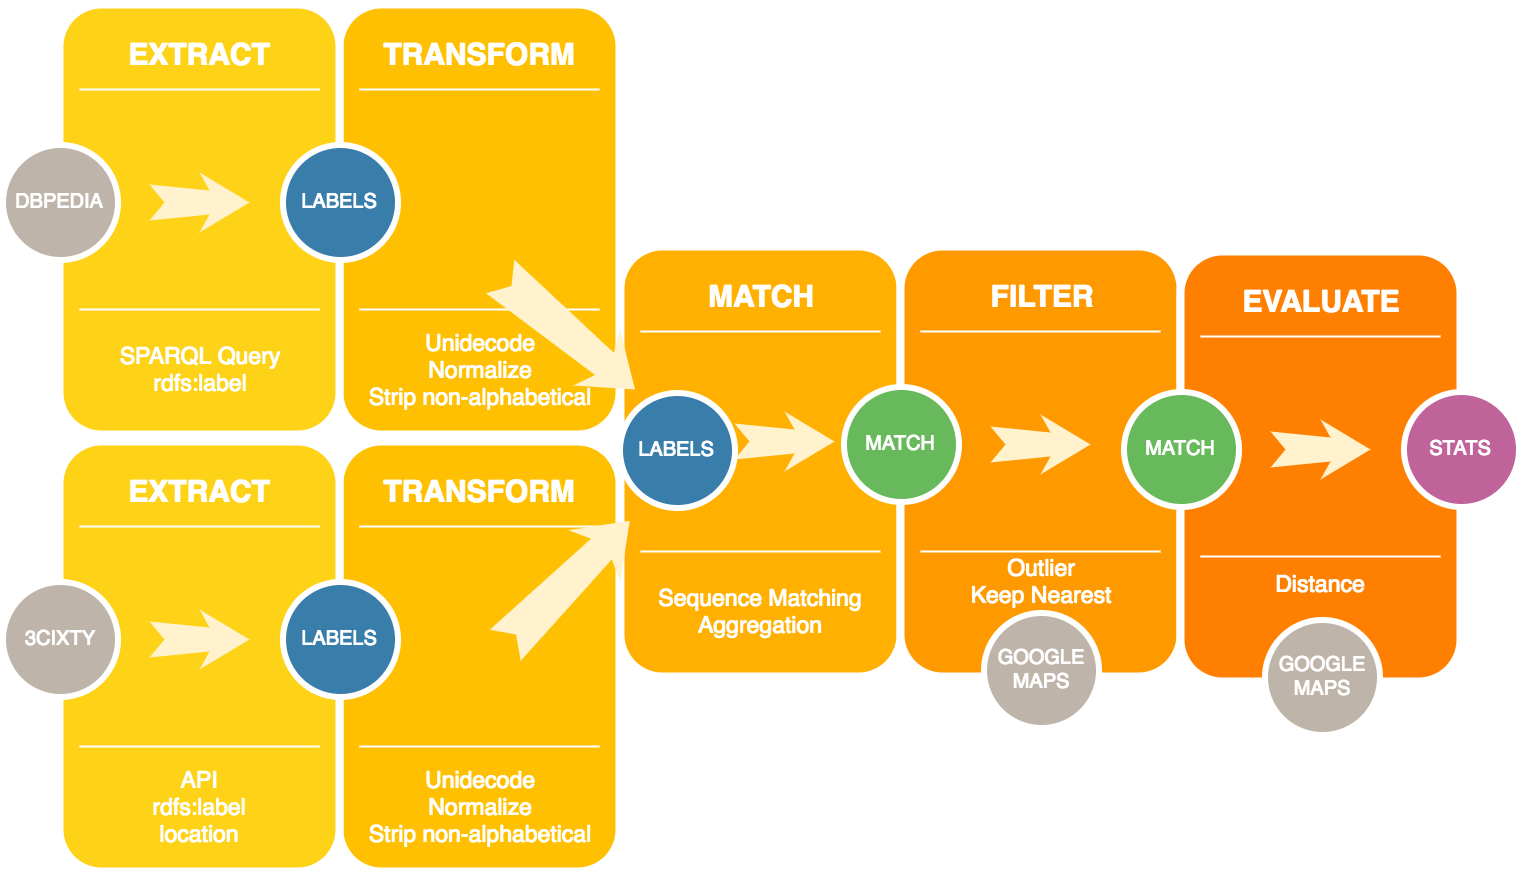
\includegraphics[width=\textwidth]{img/pipeline.png}}
%  \caption{The PoIs interlinking pipeline}
%  \label{fig:pipeline}
% \end{figure}

\subsection*{Path Finding.}
Retrieving paths between two entities has already been solved by tools such as Relfinder~\cite{heim2009relfinder} that searches the graph for possible paths with a given depth. However, increasing the depth generates both many more possible paths and makes the computation time prohibitive. In our context, the average depth is quite high, and we need in average 5-6 edges to connect a PoI of Nice to an artist. Running a query for retrieving all paths with a depth $d$ of 6 means in fact to retrieve all the triples in DBpedia, which at the time of writing is composed of 8.8 billion triples. For this reason, we developed a simplified version of Relfinder, that implements a bidirectional Breath First Search (BFS)~\cite{russell1995modern}. In practice, we search for all the paths with depth $d/2$ of 3 from both the source (PoIs) and the destination (artists) entities. Then, we intersect the two sets in order to find the common nodes, and we operate joins that recreate the full paths. This technique reduces the complexity from $O(b^d)$ to $O(b^{\sfrac{d}{2}})$, with an exponential reduction of computation times. Moreover, we decided to not consider changes in the direction of the edges until the common node. Finally, a pruning is performed in order to remove cycles (repetition of the same entity in the path) and to preserve only the shortest path for each couple of entities.

\subsection*{Path Scoring.}
Among all the possible paths between each PoI and artist, we are interested not only in the short ones, but also in paths that involve exclusive intermediate nodes, defined as the ones that minimize the generality formula:

$$gen =\frac{1}{\mid N \mid}\sum_i^Nocc(r_{i})$$

where $r_{i}$ corresponds to the $i_{th}$ resource of a path of length N and $occ(r_{i})$ to the number of its occurrences in all found paths. Given $deep_{max}$ as the biggest path depth (in our case, 7) and $len(artist,poi)$ as the considered path length, we define the similarity between a PoI and an artist using a combination of different similarity measures~\cite{meng2013review}:

$$sim(artist,poi) = 1-k(\frac{\log(len(artist,poi)-1)}{\log(2*(deep_{max} -1))})-(1-k)gen$$

We select 5 artists for each PoI with the highest similarity score.

%%%%%%%%%%%%%%%%%%%%%%%%%%%%%%%%%%%%%%%%%%%%%%%
%%%  3. CityMUS Application and Evaluation  %%%
%%%%%%%%%%%%%%%%%%%%%%%%%%%%%%%%%%%%%%%%%%%%%%%

\section{CityMUS Application and Evaluation}
\label{sec:CityMUS}

\subsection*{CityMUS Mobile Application.}
\textit{CityMUS} is a mobile web application available at \url{https://citymus.doremus.org}. The app uses the geo-location API for getting the user position. The server generates then a playlist of tracks from the artists connected to the closest 3 PoIs, with a different weights according to their distance. The Spotify APIs are used in order to display and play the tracks (\figref{fig:screenshots}.a). The user can see the path of the song that is currently played (\figref{fig:screenshots}.c) and navigate the map for discovering the songs related to other PoIs (\figref{fig:screenshots}.b).

\begin{figure}
 \centerline{
 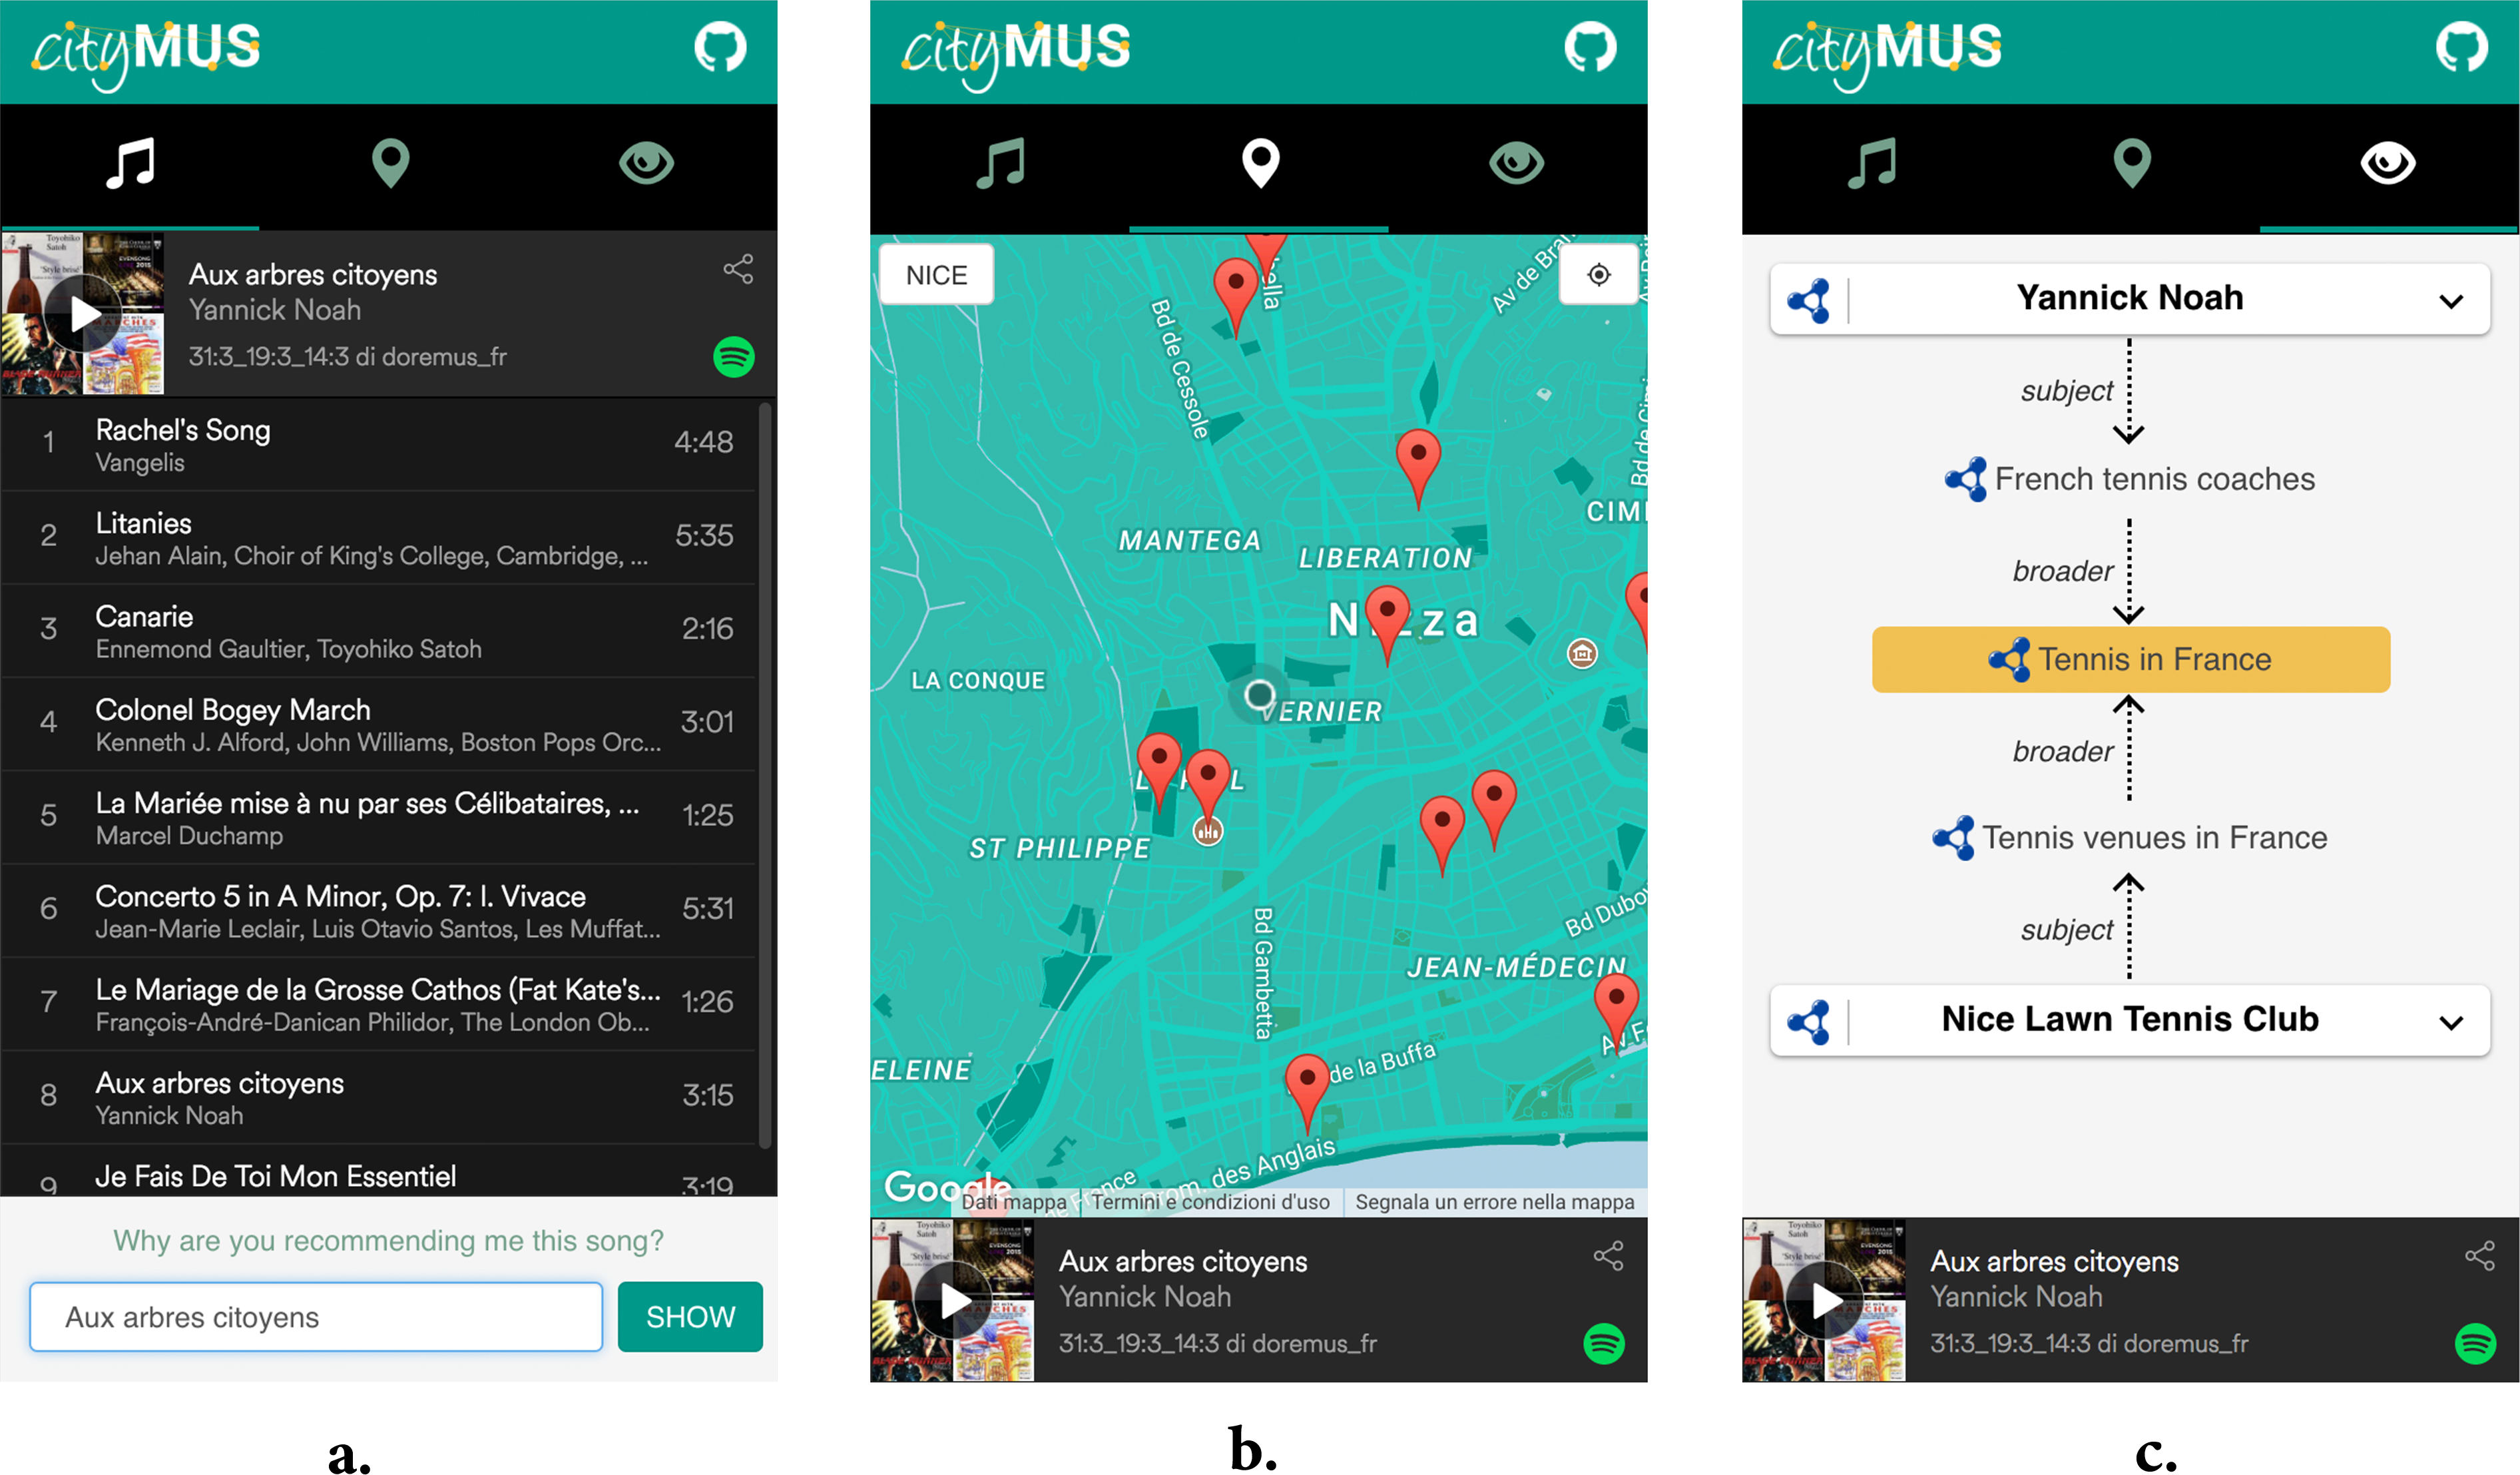
\includegraphics[width=11cm]{img/screenshots.png}}
 \caption{The \textit{CityMUS} app with its 3 views: \textbf{a.} Playlist, \textbf{b.} Map and \textbf{c.} Path Visualisation.}
 \label{fig:screenshots}
\end{figure}

\subsection*{Evaluation.}
The artists interlinking is evaluated by using as ground truth the one done by ISNI\footnote{International Standard Name Identifier, \url{http://www.isni.org}}, for which the mapping is already in the DOREMUS dataset (although not used in the interlinking task). The evaluation give us a \textit{precision} of 0.987, a \textit{recall} of 0.940 and a \textit{f-measure} of 0.963. For PoIs interlinking, we consider as correct the ones in a 250 meters distance from the one retrieved through the Google Maps API (70\% of the total).

About the path, we are interested to select specific paths, which means maximising the $gen$ function. We prune in this way lots of paths that contain very common resources (i.e. classes or reference to Nice as a city). In particular, the paths we select for \textit{CityMUS} contain resources that occur in average in just 0.001\% of all paths after the pruning, while the highest number of occurrences appears in the 0.04\% of them.

Future developments will involve the interlinking of different nodes in the musical metadata (i.e. the work itself, the genre, the historical period) that can reveal more interesting connections. A user evaluation is also planned, by adding the possibility to rate the appropiateness of a song.

\subsubsection*{Acknowledgments.}
This work has been partially supported by the French National Research Agency (ANR) within the DOREMUS Project, under grant number ANR-14-CE24-0020.

% ---- Bibliography ----
\bibliographystyle{abbrv}
\bibliography{bib-doremus}

\newpage

\end{document} 